\chapter{Introduction}

\minitoc

\section{Background}

The genome of an organism is a complete set of its DNA (Deoxyribonucleic acid), containing all the information needed to build and maintain the organism. The genome is organized into chromosomes, which are long strands of DNA further divided into genes, the basic units of heredity in living organisms. Each gene is a segment of DNA that contains instructions for making specific proteins, which constitute the structure of the organism and carry out various functions\cite{BrockBiologyMicroorganisms}.

DNA is a double-stranded molecule that encodes genetic information through the arrangement of different nucleotides, each consisting of a phosphate group, a hydroxyl group (-OH), a sugar group (deoxyribose), and a nitrogen base. The nitrogen bases differentiate the nucleotides into adenine (A), thymine (T), guanine (G), and cytosine (C), each with distinct chemical properties and serving as a unique token in the genetic vocabulary. Nucleotides in the same strand are connected by phosphorylation, where the phosphate group and the hydroxyl group combine to form a sugar-phosphate backbone. Meanwhile, the two strands are connected by hydrogen bonds between complementary nitrogen bases (A-T, G-C), forming the double helix structure of DNA. 

The sequences of the nucleotides on the DNA strands determine the genetic information of an organism, and any changes (mutations) in these sequences can have significant effects on multiple levels of the organism's biology\cite{BrockBiologyMicroorganisms}.

The ability to precisely introduce mutations of multiple types and lengths into specified locations of the genome has profound impact on medical science and the broader field of biology, and has been a long-standing goal of many researchers. It can help elucidate the function of genes and their regulatory elements, provide clinical interpretations of human gene variants, and develop new treatments for diseases, including genetic disorders and cancer\cite{petraityteGenomeEditingMedicine2021,dasCRISPRBasedTherapeutics2022,portoBaseEditingAdvances2020}. 

The discovery of the CRISPR (clustered regularly interspaced short palindromic repeats) and CRISPR-associated protein (Cas) system in the early 2000s was a major step towards this goal. The CRISPR system is originally an adaptive immune systems in bacteria and archaea providing acquired immunity against foreign nucleic acids, using RNA (ribonucleic acid) sequences as guide \cite{jiangCRISPRCas9Structures2017}. RNA sequences are single-stranded molecules that carry genetic information from DNA to the ribosome for protein synthesis. They are structurally similar to DNA but have uracil (U) instead of thymine (T) as one of the nitrogen bases. As a result, they can form hydrogen bonds with DNA, and carrying the molecules attached to the RNA to the corresponding DNA sequence\cite{BrockBiologyMicroorganisms}.
% This property forms the basis of the CRISPR system's ability to recognize and bond with foreign DNA.

The CRISPR-Cas system operates in two steps. In the adaptation step, the system acquires short sequences of foreign DNA (spacers) and derives new complementary guide RNAs from them. In the interference step, the system uses these guide RNAs to recognize and cleave foreign DNA with the help of attached Cas proteins\cite{garneauCRISPRCasBacterial2010}.

Due to its ability to recognize and introduce scissions at specific locations of the genome, the CRISPR system and a particular Cas protein, Cas9, were harnessed as a powerful tool for genome editing (Figure \ref{fig:crispr-hdr}). CRISPR-Cas9 uses a similar two-step process to introduce mutations into the genome. In the first step, the Cas9 protein is guided to the target site by a typically 20bp long single guide RNA (sgRNA) that is complementary to the target site (protospacer) adjacent to the protospacer adjacent motif (PAM) recognizable by Cas9. In the second step, the Cas9 protein introduces a double-strand break (DSB) at the target site, which is then repaired by the cell's endogenous repair machinery. 

For the desired mutation to be installed, a single or double strand DNA (ssDNA/dsDNA) donor can be provided during the second step\cite{richardsonEnhancingHomologydirectedGenome2016,jasinRepairStrandBreaks2013}. The endogenous homology directed repair (HDR) system can then use the donor DNA as template and install the intended edit\cite{hsuDevelopmentApplicationsCRISPRCas92014}. However, a competing repair pathway, non-homologous end joining (NHEJ), is more prevalent in mammalian cells and often introduces unintended insertions or deletions (indels) at the target loci\cite{changNonhomologousDNAEnd2017}. Although various improvements to the Cas9 proteins and sgRNA have been made over the years, the CRISPR-Cas9 is still mostly used to introduce disruptions into the genome rather than installing precise edits due to its high indel generation rate\cite{kantorCRISPRCas9DNABaseEditing2020,koeppelPredictionPrimeEditing2023}.

% subfigure side by side
\begin{figure}[ht]
    \centering
    \subfigure[CRISPR-Cas9 HDR]{
        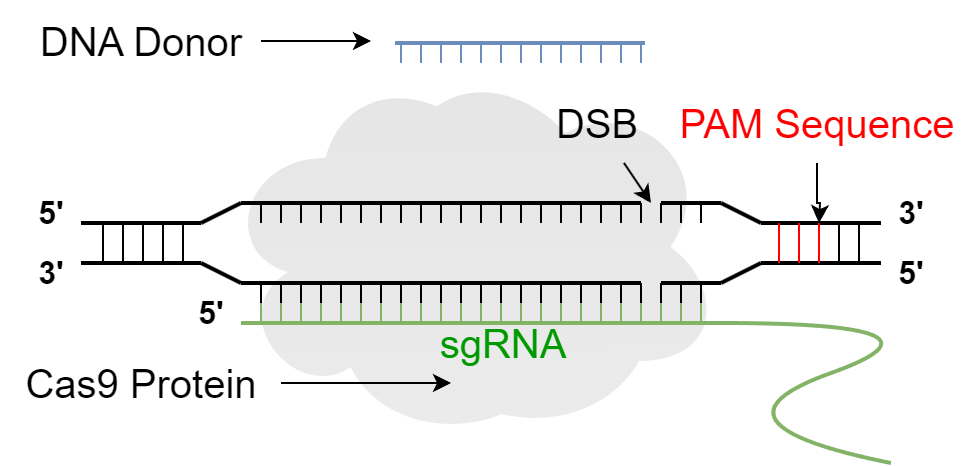
\includegraphics[width=0.46\textwidth]{dissertation-crispr-hdr.png}
        \label{fig:crispr-hdr}
    }
    \subfigure[Base Editor]{
        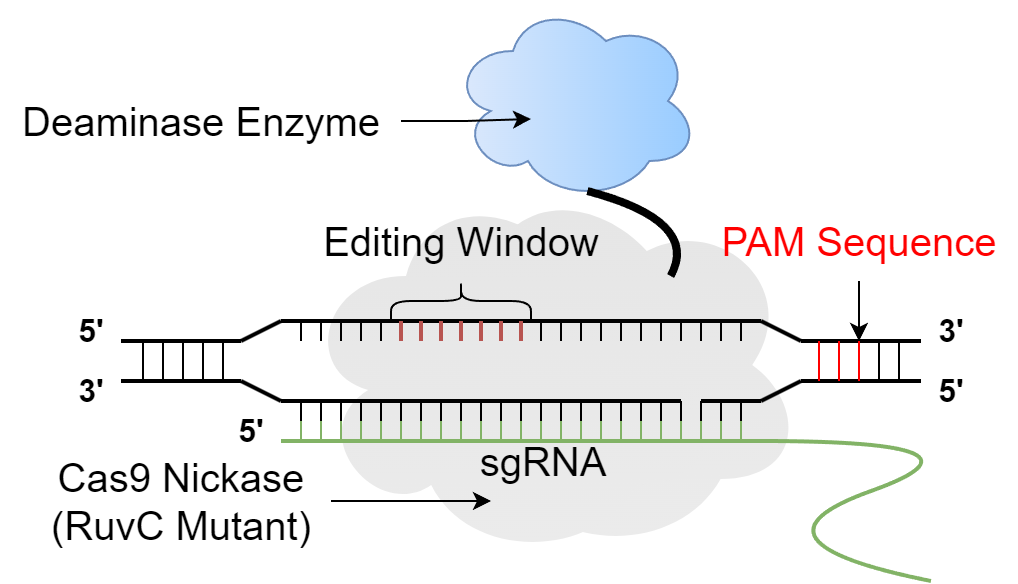
\includegraphics[width=0.46\textwidth]{dissertation-base-editor.png}
        \label{fig:base-editor}
    }
    \caption[Components of HDR and BE]{Components for \textbf{(a)} CRISPR-Cas9 HDR  and \textbf{(b)} Base Editor  systems. The directions of DNA and RNA are denoted by 3' and 5' ends, based on the numbering of carbon atoms in the deoxyribose molecule (sugar group) forming the backbone of the DNA. The 5' end refers to the end where the phosphate  group attaches to the fifth carbon atom of the deoxyribose, while the 3' end refers to the end where the hydroxyl group  attaches to the third carbon atom.}
    \label{fig:crispr-base-editor}
\end{figure}

To avoid the inefficiencies produced by DSB while still leveraging the targeting capabilities of CRISPR system, the nickase versions of Cas9 proteins were developed. Cas9 nickase is a mutated version of the Cas9 protein that only cleaves the binding (RuvC mutation) or opposite (HNH mutation) strand of the guide RNA\cite{dasCRISPRBasedTherapeutics2022}. David Liu and his team developed the base editing system that uses the RuvC mutated Cas9 nickase to introduce point mutations into the genome (Figure \ref{fig:base-editor})\cite{gaudelliProgrammableBaseEditing2017}. The base editing system consists of a fusion protein of the Cas9 nickase and a deaminase enzyme, in addition to a sgRNA that guides the fusion protein to the target site. The deaminase enzyme converts a specific nucleotide within the editing window to another base, and the Cas9 nickase introduces a nick in the non-edited strand to encourage the cell's endogenous repair machinery to use the edited strand as a template and permanently install the edit into the genome.

The base editors have been improved to be able to introduce point mutation within the editing window with relatively high efficiency\cite{portoBaseEditingAdvances2020}. However, they are only designed to introduce single-nucleotide variants into DNA or RNA, and are not capable of inserting and deleting sequences. To address this limitation in functionality and acquire a truly versatile genome editing tool, Liu's lab further developed prime editors\cite{liudavidr.SearchandreplaceGenomeEditing2019}. Prime editors are capable of introducing all 12 possible types of point mutations, as well as insertion and deletion of sequences up to a couple thousand base pairs in length\cite{linHighefficiencyPrimeEditing2021}. 

Prime editors have more complex components than base editors, consisting of a fusion protein of  SpCas9 (Streptococcus pyogenes, HNH mutated) nickase and a MMLV reverse transcriptase, as well as a prime editing guide RNA (pegRNA), illustrated in Figure \ref{fig:pe-pegrna-plasmids}. The SpCas9  nickase is a popular variant of Cas9 protein in recent years, mostly due to its high targetability (recognizing the common NGG PAM sequence, where N can be any nucleotide) and low off-target effects\cite{waltonUnconstrainedGenomeTargeting2020}. The $5'$ end of the pegRNA is very similar to the sgRNA used by base editors and CRISPR-Cas9 HDR, containing a nicking single guide RNA (ngRNA) for targeting protospacer. On the $3'$ end, however, pegRNA has a unique RNA sequence that primes and encodes the desired edit. The $3'$ sequence can be divided into two parts: the primer binding site (PBS) and the reverse transcription template (RTT) consisting of the intended edit surrounded by the left/right homology arms (LHA/RHA, RHA also called RTT overhang). As their names suggest, the PBS and RTT are used to prime the reverse transcription process, while the LHA and RHA are unedited sequences used to facilitate the integration of the edited sequence into the genome. The two ends of the pegRNA are connected by a tracrRNA scaffold sequence, which does not participate in the prime editing process. 

\section{Process of Prime Editing}

\label{sec:prime-editing-process}

Since the first generation of prime editors (PE2, PE3) was introduced in 2019, several variants have been developed, including PE4 and PE5 with the additional MLH1dn protein to inhibit the adverse mismatch repair pathway, as well as PE2-max and PE4-max with updated SpCas9 and reverse transcriptase\cite{liuPrimeEditingPrecise2023}. Despite their differences, all prime editors follow a similar multi-stage process, illustrated in \autoref{fig:pe-pegrna-plasmids} and \autoref{fig:prime-editing-process}. 

\begin{figure}
    \centering
    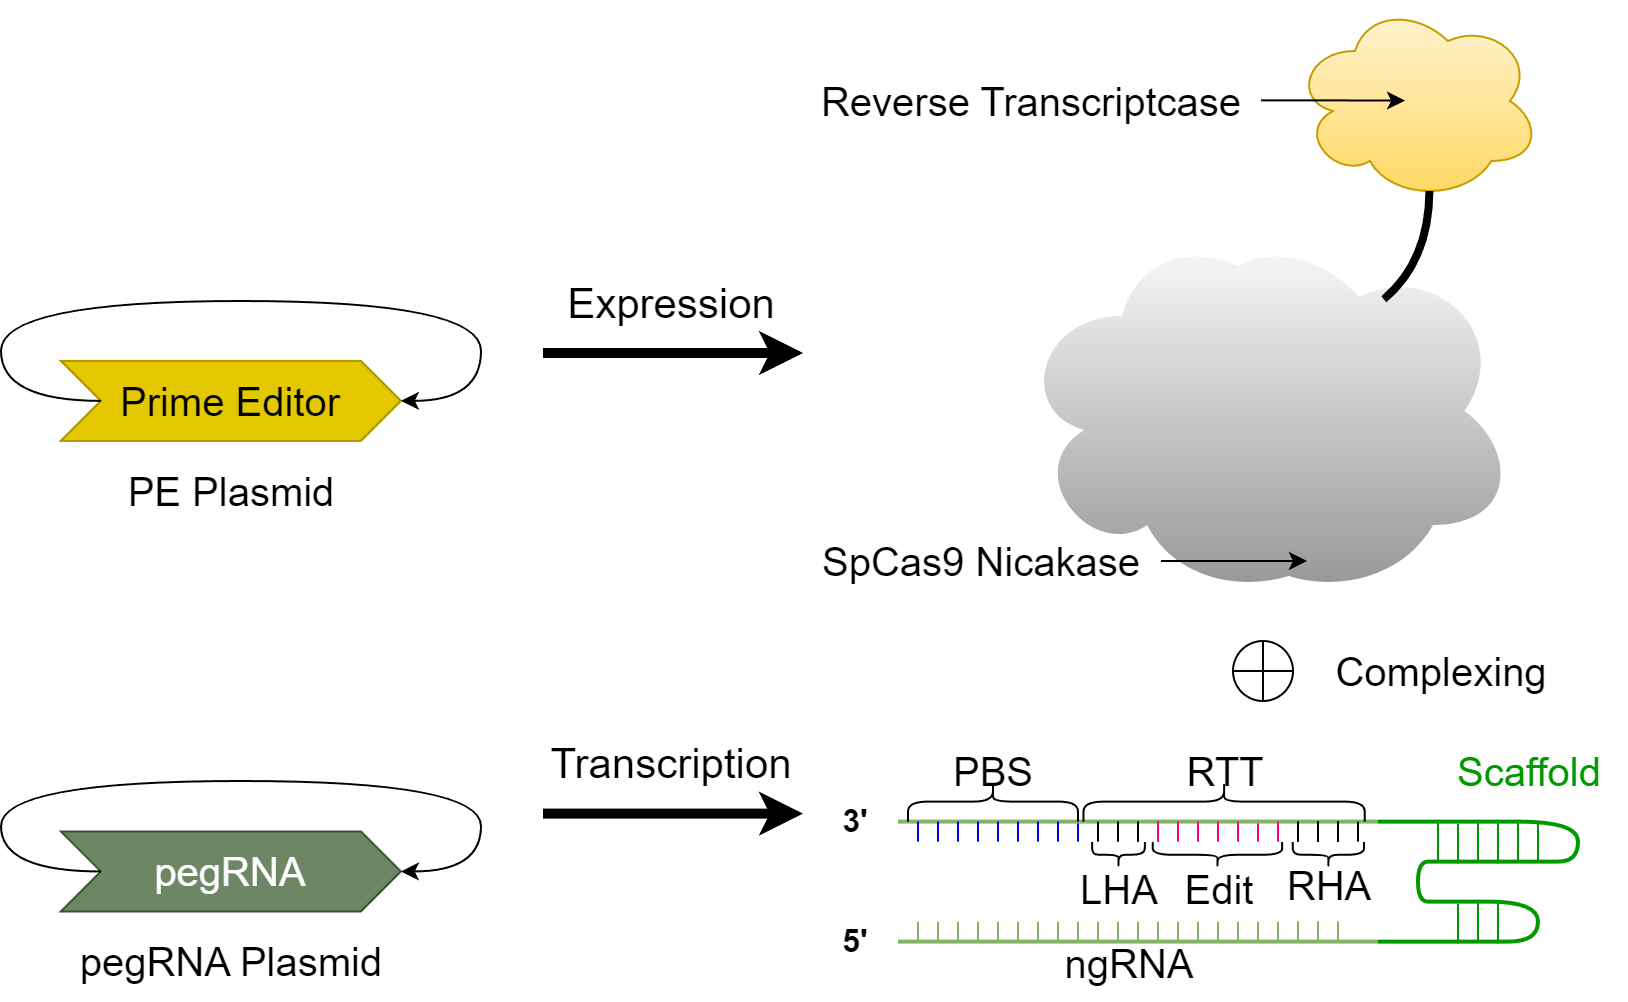
\includegraphics[width=0.85\textwidth]{dissertation-pe-pegrna-plasmids.png}
    \caption[Plasmids for Prime Editing]{The process of introducing prime editors and pegRNA into the cell. The prime editor plasmid contains the blueprint for the SpCas9 nickase and the MMLV reverse transcriptase, while the pegRNA plasmid contains the cDNA for pegRNA sequence. The sections of the plasmids not responsible for the prime editing process are omitted and replaced by an arrow. The two plasmids are transfected into the cell separately, and the prime editor complex is assembled in the cell's cytoplasm after the expression of PE and transcription of pegRNA.}
    \label{fig:pe-pegrna-plasmids}
\end{figure}

\begin{figure}[ht]
    \centering
    \subfigure[Targetting]{
        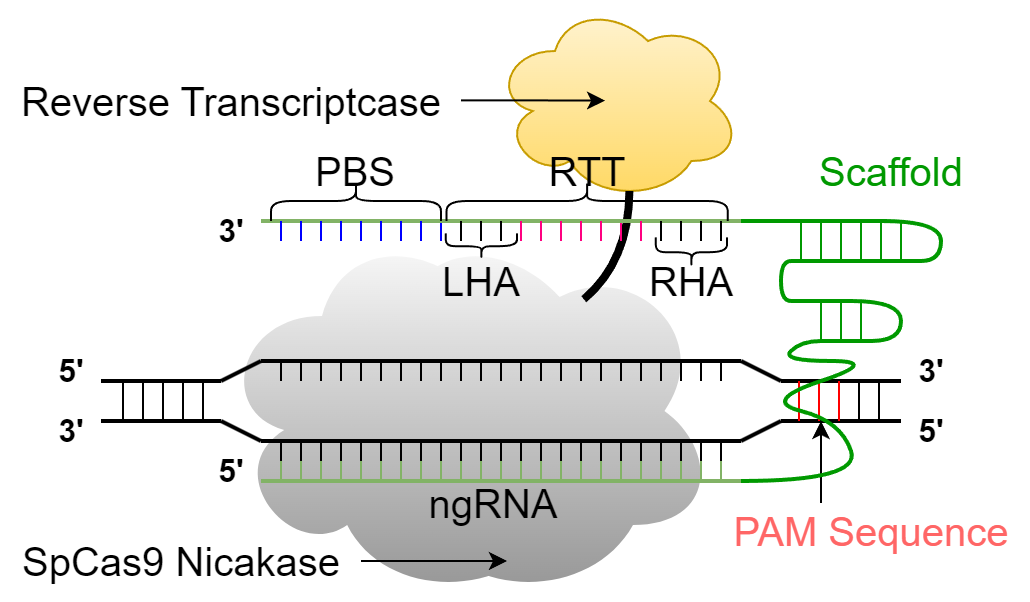
\includegraphics[width=0.46\textwidth]{dissertation-prime-editing-process-1.png}
        \label{fig:prime-editor}
    }
    \subfigure[Nicking]{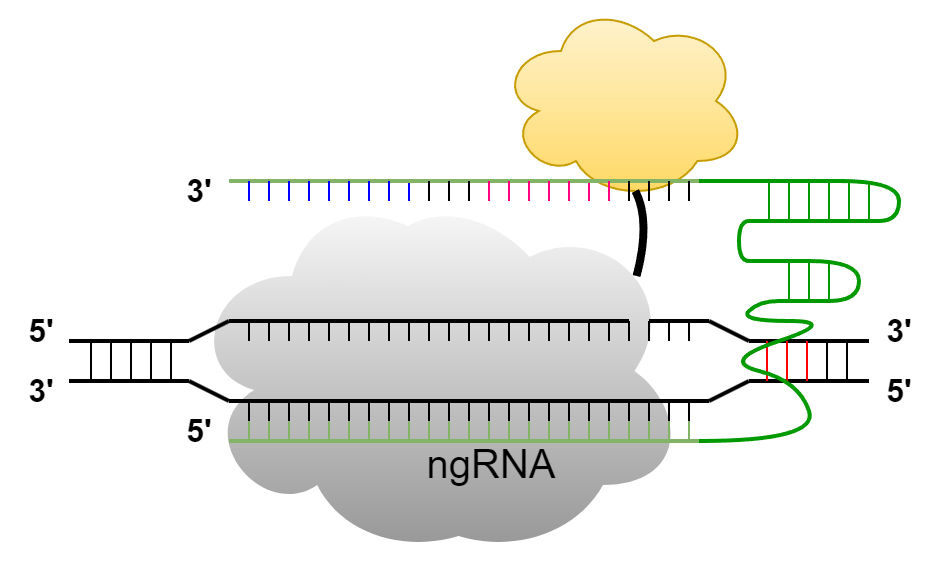
\includegraphics[width=0.46\textwidth]{dissertation-prime-editing-process-2.png}}
    \subfigure[PBS Hybridization]{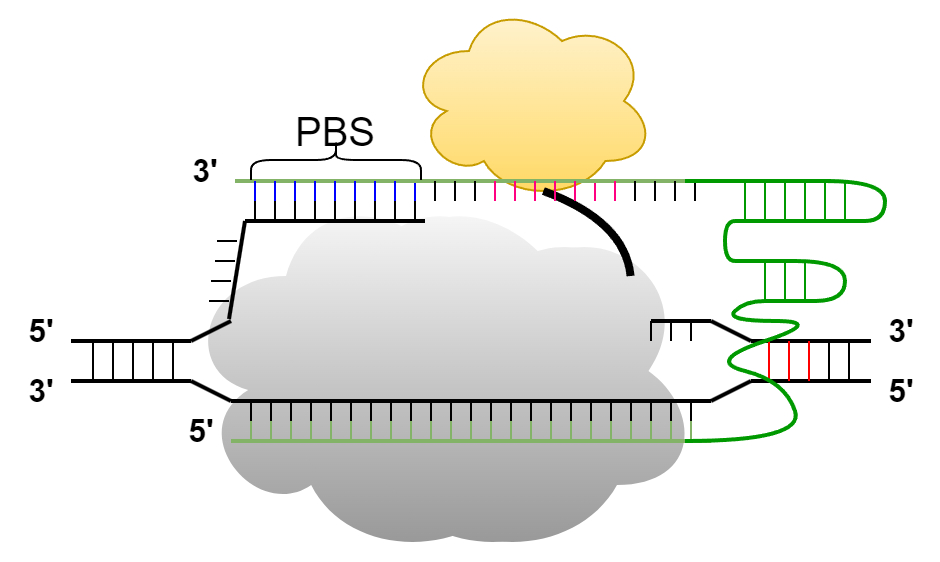
\includegraphics[width=0.46\textwidth]{dissertation-prime-editing-process-3.png}}
    \subfigure[Reverse Transcription]{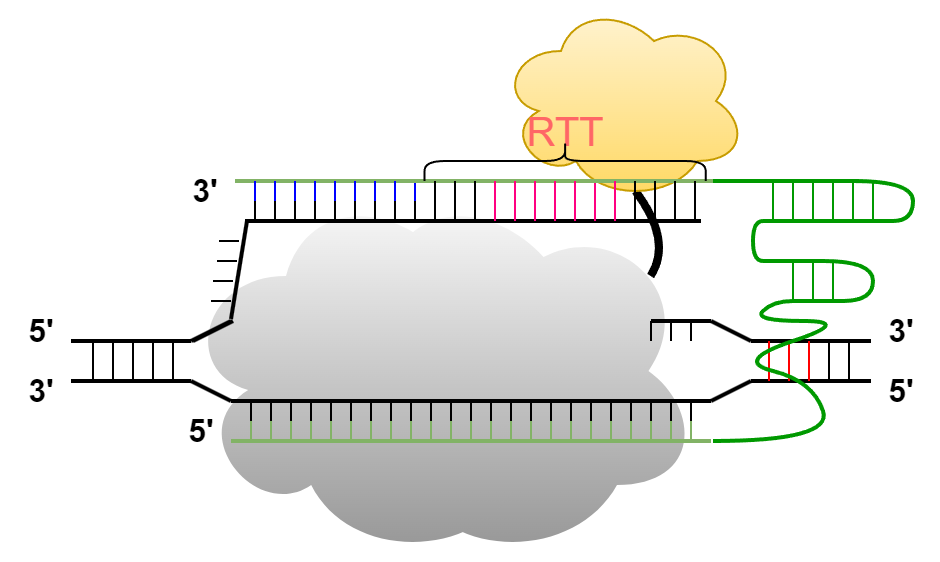
\includegraphics[width=0.46\textwidth]{dissertation-prime-editing-process-4.png}}
    \subfigure[Flap Excision]{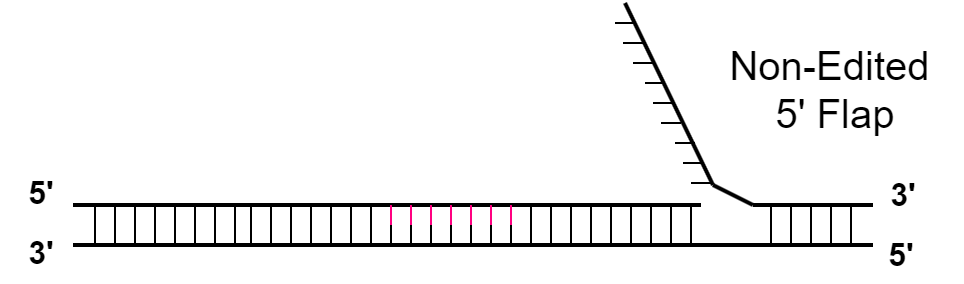
\includegraphics[width=0.46\textwidth]{dissertation-prime-editing-process-5.png}}
    \subfigure[Completion]{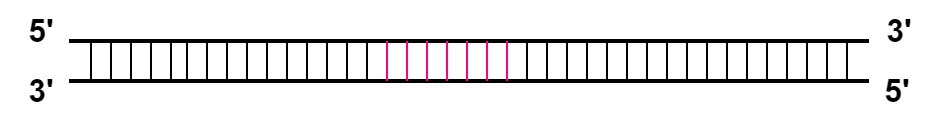
\includegraphics[width=0.46\textwidth]{dissertation-prime-editing-process-6.png}}
    \caption[Process of prime editing]{Process of prime editing after successful expression and transcription of PE and pegRNA plasmids. \textbf{(a)} ngRNA binds to the target DNA loci (protospacer) directly upstream of PAM; \textbf{(b)} SpCas9 introduces nick 3-4 bp upstream of PAM; \textbf{(c)} The now exposed strand hybridizes with the PBS sequence in the pegRNA; \textbf{(d)} The RTT in the pegRNA is reverse transcribed into the target DNA; \textbf{(e)} The edited strand anneals to the non-edited strand; \textbf{(f)} The endogenous repair machinery incorporates the edited strand into the genome.}
    \label{fig:prime-editing-process}
\end{figure}

Before the prime editing can start, the prime editor components need to be delivered into the cell. pegRNA and prime editor proteins are typically delivered separately as plasmids, which are double stranded circular DNA molecules that can be easily replicated and transcribed by the transfected cells. The pegRNA plasmids are transcribed into RNA by the cell's endogenous transcription machinery, and the prime editor proteins are expressed by the cell's ribosome. The two components then assemble into the prime editor complex in the cell's cytoplasm (the fluid inside the cell), ready to locate the target loci and begin the editing process\cite{liudavidr.SearchandreplaceGenomeEditing2019}. 

The prime editing process starts with the denaturing (separation of the two strands) of target DNA loci. This allows ngRNA to bind to the complementary sequence immediately upstream of the protospacer adjacent motifs (PAM) required for successful annealing (binding of two complementary strands of DNA or RNA). The Cas9 nickase can then nick the exposed strand of the target DNA, creating a floating 3' end that can be used as a primer for the reverse transcription process. Finally, the PBS sequence in the pegRNA binds to the floating 3' end, priming the reverse transcription of the RTT.

After the transcription finishes, both the reverse transcribed 3' flap and non-edited 5' flap could anneal to the protospacer, and would result in a equilibrium of 3' and 5' flaps. If the edited 3' flap is excised, target would not be edited and can be processed again with prolonged editing. If the 5' flap is correctly excised, then we proceed to the final step where the endogenous cellular repair system permanently incorporates the edited strand into the genome by repairing the mismatched base pairs. Similar to the mechanism exploited by base editing, PE3 and PE5 have an additional sgRNA that guides the PE enzyme to nick the non-edited strand, encouraging the cell to use the edited strand as a template for repair\cite{liudavidr.SearchandreplaceGenomeEditing2019}.

\section{In-silico Prediction of Prime Editing Outcome}

\label{sec:motivation}

More than 6,000 disorders are known to be caused by various types of mutations in the genome, with around 300 new genetic disorders being discovered each year\cite{petraityteGenomeEditingMedicine2021}. Due to its versatility, prime editing has the potential to correct up to 90\% of these disorder-inducing mutations\cite{kantorCRISPRCas9DNABaseEditing2020}, and the coverage is still increasing with new SpCas9 variants that have less and less PAM sequence constraints\cite{waltonUnconstrainedGenomeTargeting2020}. However, for prime editors to be useful in treating human diseases in clinical setting, it is crucial to have the highest possible accuracy with minimal off-target effects during the edits. 

Although prime editors have been shown to have high efficiency and low off-target effects in many cell lines, the efficiency of prime editing can vary significantly depending on the target loci and the pegRNA design\cite{liudavidr.SearchandreplaceGenomeEditing2019}. Empirical approaches have been used to find the optimal prime editor guide given a target edit, which involves testing a large number of combinations of ngRNA, PBS and RTT sequences repeatedly to find the optimal combination that yields the highest editing efficiency.

Empirical optimization is a laborious and time consuming process even for simpler editing tools such as base editors. With the more complicated process of prime editing, the search space is even larger. The lack of efficient optimization process can severely limit prime editors' practicality in the clinical setting, especially in territories with an existing shortage of medical workers. As a result, in-silico optimization methods are highly desirable and has garnered the interest of many researchers. 

Existing in-silico methods can be divided into two catagories: hypothesis driven models that use hard-coded rules to calculate the efficiency of a given edit\cite{hsuPrimeDesignSoftwareRapid2021,hwangPEDesignerPEAnalyzerWebbased2021}, and learning-based models that use machine learning to predict the editing outcome. 
The learning-based methods can be further divided into another two groups: the conventional machine learning methods that use hand-crafted features extracted from the sequence and prime editors\cite{liEasyPrimeMachineLearning2021,koeppelPredictionPrimeEditing2023}, as well as the deep learning methods that use the raw sequence data as part of their input\cite{yuPredictionEfficienciesDiverse2023,kimPredictingEfficiencyPrime2021, mathisPredictingPrimeEditing2023}. 

Each category has its own strengths and weaknesses in performance and efficiency. Hypothesis driven and conventional machine learning algorithms are more efficient to train due to the much smaller input size and the lower complexity of the computation. However, hypothesis based methods often struggle to unbiasedly optimize the weights attributed to each feature\cite{liEasyPrimeMachineLearning2021}, while conventional machine learning algorithms loses the DNA context data that can be informative to prime editor optimization. 

The deep learning methods require a much larger dataset and significantly more computational resource during training. They also need more expertise to design and tune, and are more prone to overfitting due to the large number of parameters. However, their superior performance in the prime editing efficiency prediction task has been convincingly demonstrated by a number of models in recent years.

% TODO: overview of DeepPE, DeepPrime, PRIDICT 1 and 2

\subsection{DeepPE and DeepPrime convolutional neural network}


\begin{figure}
    \centering
    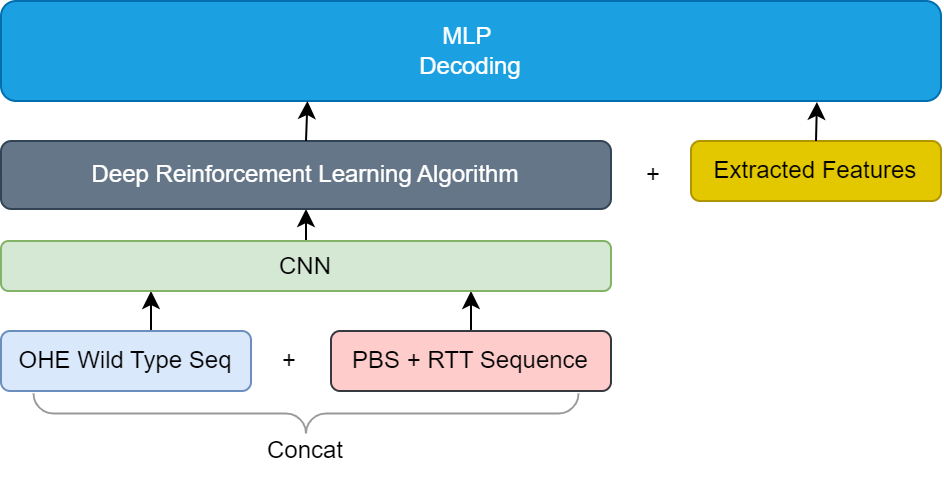
\includegraphics[width=0.7\textwidth]{DeepPE-simplified.png}
    \caption[DeepPE architecture]{DeepPE architecture. The input to the CNN is the one-hot encoded wild type and mutated DNA sequences concatenated with the extension RNA sequence. A deep reinforcement learning model was used here instead of a pooling layer to maintain local context information from the CNN. The output of the CNN is concatenated with the extracted features from the pegRNA sequence and the target site, and fed into the final MLP to predict the editing efficiency. }
    \label{fig:deeppe}
\end{figure}


DeepPE (\autoref{fig:deeppe}) is one of the earliest attempts at leveraging deep learning to achieve above par performance in predicting prime editing outcomes\cite{kimPredictingEfficiencyPrime2021}. It is a convolutional neural network (CNN) that takes the stacked one-hot encoded wild-type/mutated DNA sequences, the $3'$ extension portion of the pegRNA sequence, as well as a number of extracted features (RTT length, Protospacer melting temperature etc.) as input. Despite its simple architecture, DeepPE managed to outperform the conventional machine learning models in terms of Pearson's r and Spearman's $\rho$ between predicted and true editing efficiencies. This indicates that compared to using the extracted features alone, the deep learning model is able to better capture the complex interactions between the sequence data and the editing efficiency. However, DeepPE is limited in the types of edits it can predict, with the base model only capable of predicting the efficiency of G to C replacement at 5 bp downstream of the nick.

Building on the demonstrated capability of CNNs in this task, Kim et al. further developed DeepPrime, leveraging a much larger dataset and an improved architecture design\cite{yuPredictionEfficienciesDiverse2023}.
Noticing that stacking the additional PBS-RTT sequence did not improve the performance of DeepPE, DeepPrime only uses the wild type and mutated sequences as input to the deep learning model. Additionally, instead of directly concatenating the output of the CNN with the extracted features, a MLP (Multi-Layer Perceptron) module is used to first process the extracted features.
The outputs of the two modules are then concatenated and fed into a separate MLP to predict the editing efficiency.

\begin{figure}
    \centering
    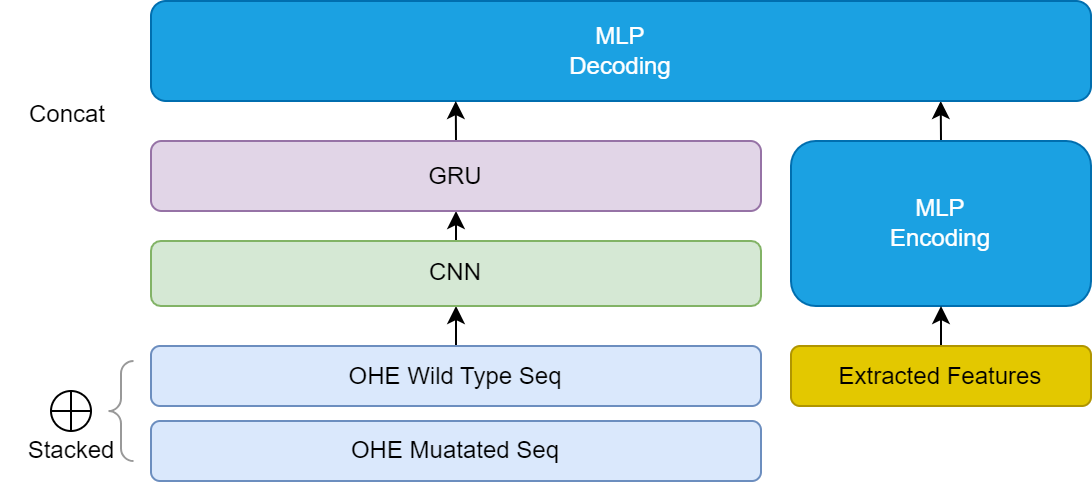
\includegraphics[width=0.85\textwidth]{DeepPrime-simplified.png}
    \caption[DeepPrime architecture]{DeepPrime architecture, updated from DeepPE. The CNN now uses a more conventional pooling layer, followed by a RNN GRU (Gated Recurrent Unit). The convolutional and recurrent layers take the stacked one-hot encoded wild type and mutated DNA sequences as input, and the output is concatenated with the extracted features processed by a MLP module. The concatenated output is then fed into another MLP to predict the editing efficiency.}
    \label{fig:deepprime}
\end{figure}

DeepPrime achieved far superior performance than DeepPE, while at the same time, one single model can now predict all types of edits for a cell line and prime editor pair in the dataset. This enabled the training process to take advantage of the shared features between different edits (further enhancing performance) and significantly improved the ease of use.

\subsection{PRIDICT 1 and 2 bidirectional GRU}

At around the same time DeepPrime was published, an RNN (Recurrent Neural Network) based model PRIDICT was developed by Mathis et al from the Schwank lab at the University of Zurich\cite{mathisPredictingPrimeEditing2023}. PRIDICT uses a bidirectional GRU (Gated Recurrent Unit) to process the concatenated wild type and mutated sequence, whose output is pooled by a pair of global (whole sequence) and local (RTT region) attention(\autoref{fig:pridict}). Similar to DeepPrime, the features are first encoded using a MLP. The outputs of the two models are then concatenated and fed into the final MLP to predict the editing efficiency.

\begin{figure}
    \centering
    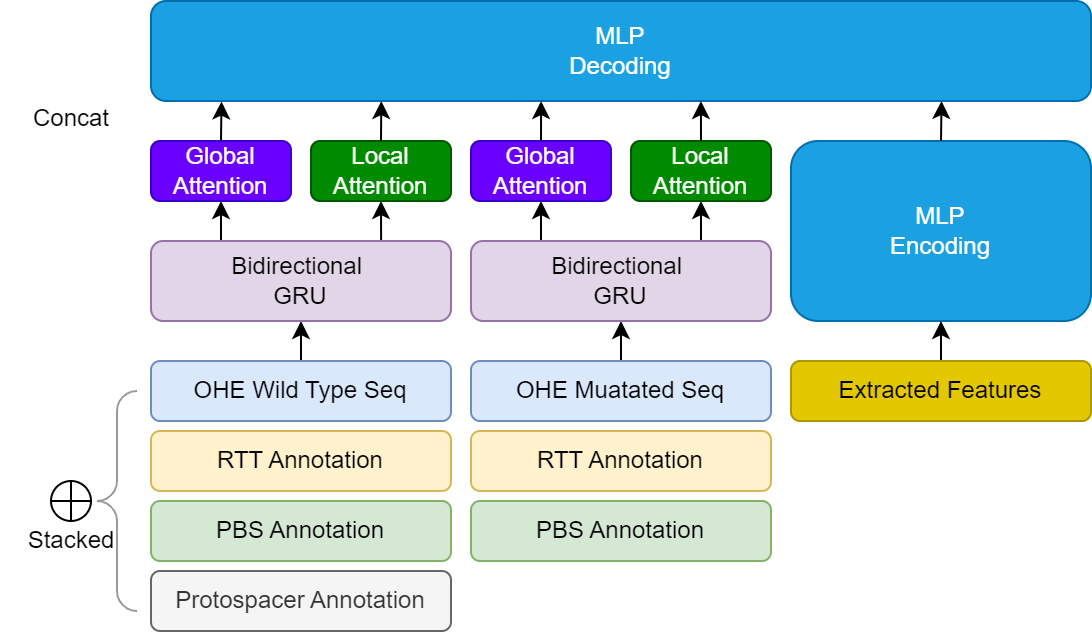
\includegraphics[width=0.85\textwidth]{pridict-simplified.png}
    \caption[PRIDICT architecture]{PRIDICT architecture. The input to the RNN is the one-hot encoded wild type and mutated DNA sequences, stacked with RTT, PBS, Protospacer(only for wild type) annotations. The annotation sequences are boolean sequences that indicate the functionality of each nucleotide in the sequence. The output of the RNN is processed by two attention heads, a global one that processes the entire sequence and a local one that masks out all regions other than RTT before processing.}
    \label{fig:pridict}
\end{figure}

This RNN based model is able to predict the efficiency of prime editing outcomes with up to 0.8 Pearson's r on their dataset, and is reported to be on par with the performance of DeepPrime.

Encouraged by the success of the bidirectional RNN, the PRIDICT 2 model was soon developed by applying minor tweaks to the architecture as well as the data preprocessing steps and achieved even higher performance\cite{mathisMachineLearningPrediction2024}. More importantly, thanks to the far more diverse edits in the dataset with much longer inserts and deletes than the up to 3bp long edits in DeepPrime, PRIDICT 2 is more capable in the laboratory setting where insertion and deletions are often reaching hundreds of base pairs in length\cite{liuPrimeEditingPrecise2023}.

\section{Study Objective}

The development of these models has noticeably advanced the field of prime editing, and demonstrated the potential of deep learning in predicting the efficiency of prime editing outcomes. This inspired me to further explore the capabilities of deep learning in this task, and to develop a model that can predict the efficiency of prime editing outcomes with on par or even superior performance than the existing methods.

% The study will begin with the construction of a benchmarking dataset of prime editing outcomes from the literature, incorporating 23 datasets derived from two different studies. The dataset will be used to train and evaluate the performance of the existing models as well as the new models developed in this study.

The study will begin with the construction of ensembles of the existing solutions, including DeepPrime and PRIDICT, to leverage their individual strengths and create more robust models. Several ensemble methods will be implemented and evaluated, including weighted average, bagging, and boosting.

Additionally, the study will also explore the possibility of applying the transformer model, a deep learning model highly effective in sequence-to-sequence tasks, to the prime editing efficiency prediction task. 

The best performing model will be presented as a web application that can be used by researchers with no machine learning experience to predict the efficiency of prime editing outcomes for an intended edit.